\documentclass[english,9pt,aspectraio=169]{beamer}
\usepackage{etex}
\usetheme{uzhneu-en-informal}
%\usepackage{uarial}
\usepackage[T1]{fontenc}
\usepackage[utf8]{inputenc}
\RequirePackage{graphicx,ae}
\usepackage{bm}
\usepackage{fancybox,amssymb,color}
\usepackage{pgfpages}
\usepackage{booktabs}
\usepackage{verbatim}
\usepackage{animate}
\usepackage{numprint}
\usepackage{dsfont}
\usepackage{tikz}
\usepackage{amsmath,natbib}
\usepackage{mathbbol}
\usepackage{babel}
\usepackage{SweaveSlides}
\usepackage{multicol}
\usepackage{xcolor}


\usetheme{uzhneu-en-informal}
\DeclareMathOperator{\po}{Poisson}
\DeclareMathOperator{\G}{Gamma}
\DeclareMathOperator{\Be}{Beta}
\DeclareMathOperator{\logit}{logit}
\def\n{\mathop{\mathcal N}}

\definecolor{Gray}{RGB}{139,137,137}
\definecolor{darkred}{rgb}{0.8,0,0}
\definecolor{Green}{rgb}{0,0.8,0.3}
\definecolor{Blue}{rgb}{0,0,1}
\def\myalert{\textcolor{darkred}}
\def\myref{\textcolor{Gray}}
\setbeamercovered{invisible}

\renewcommand{\baselinestretch}{1.2}
\beamertemplateballitem
\DeclareMathOperator{\cn}{cn} % Copy number
\DeclareMathOperator{\ccn}{ccn} % common copy number
\DeclareMathOperator{\p}{p} % common copy number
\DeclareMathOperator{\E}{E} % common copy number
\DeclareMathOperator{\given}{|} % common copy number
\def\given{\,|\,}
\def\na{\tt{NA}}
\def\nin{\noindent}
\pdfpageattr{/Group <</S /Transparency /I true /CS /DeviceRGB>>}
\def\eps{\varepsilon}

\renewcommand{\P}{\operatorname{\mathsf{Pr}}} % Wahrscheinlichkeitsmaß
\def\eps{\varepsilon}
\def\logit{\text{logit}}
%\newcommand{\E}{\mathsf{E}} % Erwartungswert
\newcommand{\Var}{\text{Var}} % Varianz
\newcommand{\NBin}{\text{NBin}}
\newcommand{\Po}{\text{Po}}
\newcommand{\N}{\mathsf{N}}

\newcommand{\ball}[1]{\begin{pgfpicture}{-1ex}{-0.65ex}{1ex}{1ex}
\usebeamercolor[fg]{item projected}

{\pgftransformscale{1.75}\pgftext{\normalsize\pgfuseshading{bigsphere}}}
{\pgftransformshift{\pgfpoint{0pt}{0.5pt}}
\pgftext{\usebeamerfont*{item projected}{#1}}}
\end{pgfpicture}}%
\usepackage{multicol}
\newcommand{\ballsmall}[1]{\begin{pgfpicture}{-1ex}{-0.65ex}{.2ex}{.2ex}

{\pgftransformscale{1}\pgftext{\normalsize\pgfuseshading{bigsphere}}}
{\pgftransformshift{\pgfpoint{0pt}{0.5pt}}
\pgftext{\usebeamerfont*{item projected}{#1}}}
\end{pgfpicture}}%




\begin{document}

\fboxsep5pt

{
\title[]{ \centering \Huge Kurs Bio144: \\
Datenanalyse in der Biologie}%\\[.3cm]
\author[Stefanie Muff, Owen L.\ Petchey]{\centering Stefanie Muff (Lecture) \& Owen L.\ Petchey (Exercises)}
%\institute[]{Institute of Social and Preventive Medicine \\ Institute of Evolutionary Biology and Environmental Studies}
\date[]{Week 2: Simple linear regression\\ 2./3. March 2017}


\maketitle
}


\frame{\frametitle{Overview}
\begin{itemize}
\item Introduction of the linear regression model
\item Parameter estimation
\item Goodness of the model: Correlation and $R^2$
\item Tests and confidence intervals
\item Confidence and prediction ranges
\end{itemize}
}



\frame{\frametitle{Course material covered today}
\begin{itemize}
\item Chapter 2 of \emph{Lineare Regression}, p.7-20 (Stahel script), or chapters 13.1 - 13.4 in the Stahel book ``Statistische Datenanalyse''.
\item Something from \emph{The New Statistics with R}
\end{itemize}
}


\frame[containsverbatim]{\frametitle{The body fat example}
Remember: Aim is to find prognostic factors for body fat, without actually measuring it. \\
Even simpler question: How good is BMI as a predictor for body fat?

\begin{center}

\setkeys{Gin}{width=0.5\textwidth}
\begin{Schunk}
\begin{Sinput}
> plot(bodyfat ~ bmi,d.bodyfat,xlab="bmi (x)", ylab="body fat (y)")
\end{Sinput}
\end{Schunk}
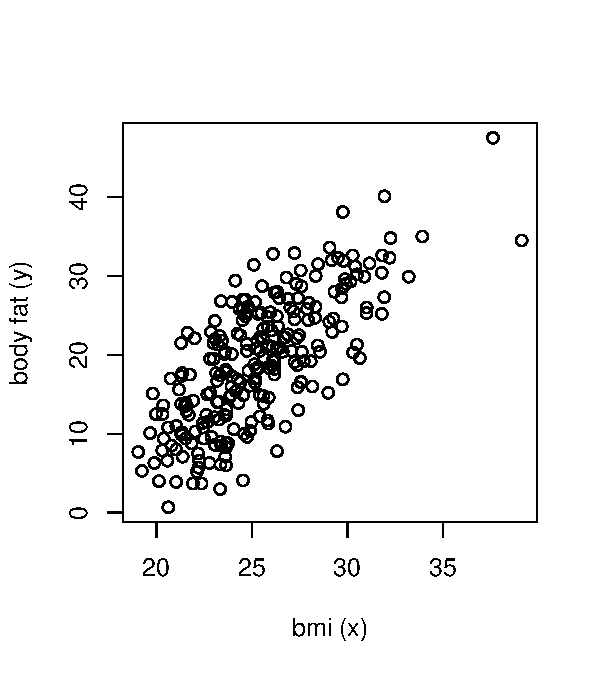
\includegraphics{Bio144_2017_week2-002}
\end{center}

}


\frame[containsverbatim]{\frametitle{Linear relationship}
\begin{itemize}
\item The most simple relationship between an \emph{explanatory variable} ($X$) and a \emph{target/outcome variable} ($Y$) is a linear relationship. All points $(x_i,y_i)$, $i= 1,\ldots, n$, on a  straight line follow the equation
$$y_i = \alpha + \beta x_i\ .$$

\item Here, $\alpha$ is the \myalert{axis intercept} and $\beta$ the \myalert{slope} of the line. 
$\beta$ is also denoted as the regression coefficient of $X$.\\[4mm]


\item If $\alpha=0$ the line goes through the origin.
\end{itemize}
}



\frame[containsverbatim]{\frametitle{}

But which is the ``true'' or ``best'' line?
\vspace{-6mm}
\begin{center}
\setkeys{Gin}{width=0.6\textwidth}
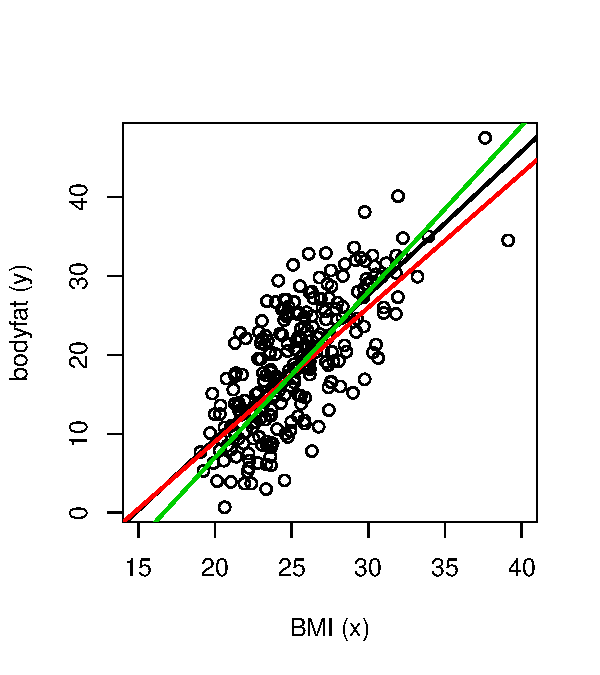
\includegraphics{Bio144_2017_week2-003}
\end{center}
}

\frame[containsverbatim]{\frametitle{}
It is obvious that another realization of the data (other 241 males) would lead to a slightly different picture.\\[4mm]

$\Rightarrow$ The model should take this into account! \\[4mm]

{\bf Solution:} Add an \myalert{error term} $E_i$ to the predictor
$$(body fat)_i = \alpha + \beta \cdot bmi_i + E_i  \ ,$$
where $E_i$ treated as a random variable with a \myalert{normally distributied}
$$E_i ~\sim \N(0,\sigma_E^2) \quad \text{for } i = 1,\ldots, n \ .$$

This is a \myalert{model} for $bodyfat$ given $bmi$.
The assumption is that the target value $bodyfat_i$ is the sum of a predicted value ($\alpha + \beta \cdot bmi_i$) plus an error term $E_i$.

}

\frame{\frametitle{The simple linear regression model}
Generally:
\colorbox{lightgray}{\begin{minipage}{10cm}
The linear regression model for the data $\bm{y}=(y_1,\ldots,y_n)$ given $\bm{x}=(x_1,\ldots,x_n)$ is

%
$$y_i = \alpha + \beta x_i + E_i \ , \qquad E_i \sim \N(0,\sigma_E^2) \  \text{independent}.$$
\end{minipage}}
~\\[2mm]
The assumption is that
$$y_i \quad= \quad \underbrace{\text{\ prediction\ }}_{\alpha + \beta x_i} \quad + \quad \underbrace{\text{\ error\ }}_{E_i}$$

\vspace{2mm}
Note:

\begin{itemize}
\item The model for $\bm{y}$ given $\bm{x}$ has \myalert{three parameters}: $\alpha$, $\beta$ and $\sigma_E^2$ .
\item $\bm{x}$ is the \myalert{independent} or \myalert{explanatory} variable.
\item $\bm{y}$ is the \myalert{dependent} or \myalert{outcome} variable. \\
\end{itemize}


}

\frame{\frametitle{}
This is a general approach in statistics:\\[6mm]
\begin{itemize}
\item Formulate a model and modelling assumptions that seem plausible for your data. A model emerges in our mind.\\[2mm]
\item Estimate the parameters.\\[2mm]
\item Only now it is a \emph{specific} model.
\end{itemize}
}

\frame{\frametitle{Visualization of regression assumptions}

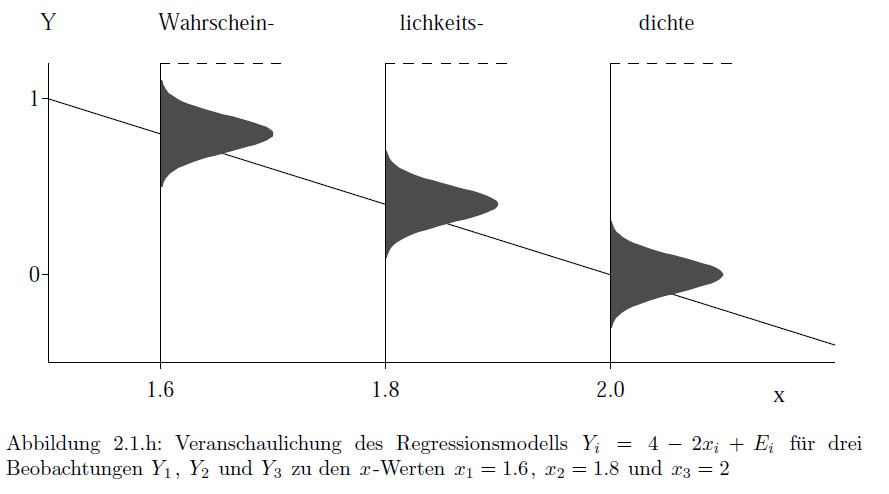
\includegraphics[width=11cm]{pictures/regrAssumptions.jpg}
}

\frame[containsverbatim]{\frametitle{Insight from data simulation}
{\scriptsize (Simulation are \emph{always} a great way to understand statistics!!)}\\[2mm]

Generate an independent (explanatory) variable $\bm{x}$ and {\bf two} samples of a dependent variable $\bm{y}$ assuming that
$$y_i = 4 - 2x_i + E_i \ , \quad E_i\sim \N(0,0.5^2) \ .$$


\begin{center}
\setkeys{Gin}{width=0.4\textwidth}
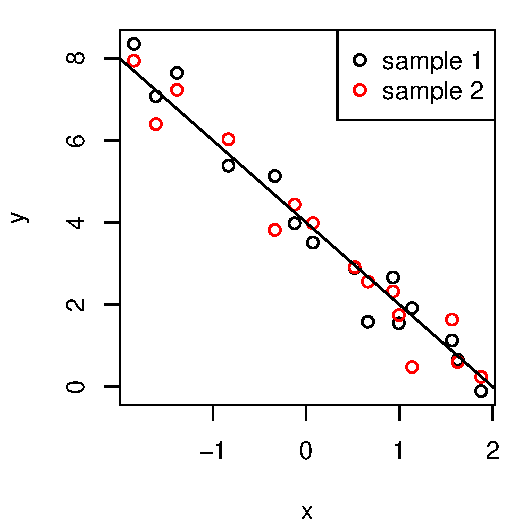
\includegraphics{Bio144_2017_week2-004}
\end{center}
Note the different y-coordinates for the two samples.

}


\frame[containsverbatim]{\frametitle{}
Or one larger sample:
\setkeys{Gin}{width=0.6\textwidth}
\begin{center}
\begin{Schunk}
\begin{Sinput}
> par(mfrow=c(1,1))
> x <- rnorm(100)
> y <- 4 - 2*x + rnorm(100,0,sd=0.5)
> plot(x,y);abline(c(4,-2))
\end{Sinput}
\end{Schunk}
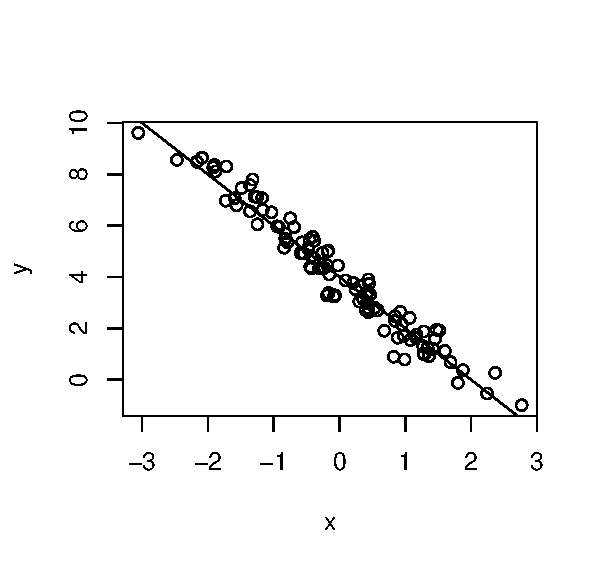
\includegraphics{Bio144_2017_week2-005}
\end{center}

Random variation is always present. This leads us to the next question.
}



\frame{\frametitle{Parameter estimation}
Remember: There are \myalert{three parameters} $\alpha$, $\beta$ and $\sigma_E^2$ that want to be estimated.\\[4mm]

\begin{itemize}
\item {\bf Problem:} For more than two points there is generally no perfectly fitting line.\\[4mm]
\item {\bf Aim:} We want to find the best fitting line.\\[4mm]
\item {\bf Idea:} Minimize the deviations between the points and the line.\\[4mm]
\end{itemize}

But how?

}



\frame{\frametitle{Should we minimize these distances...}

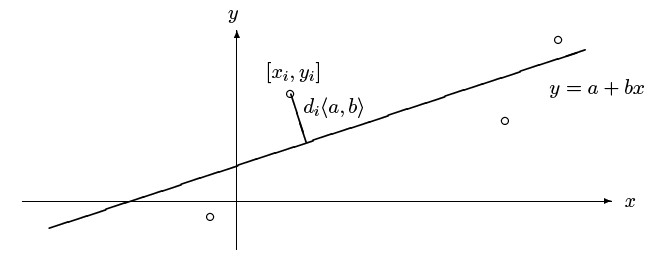
\includegraphics[width=11cm]{pictures/orthRegr.jpg}
}


\frame{\frametitle{... or these?}

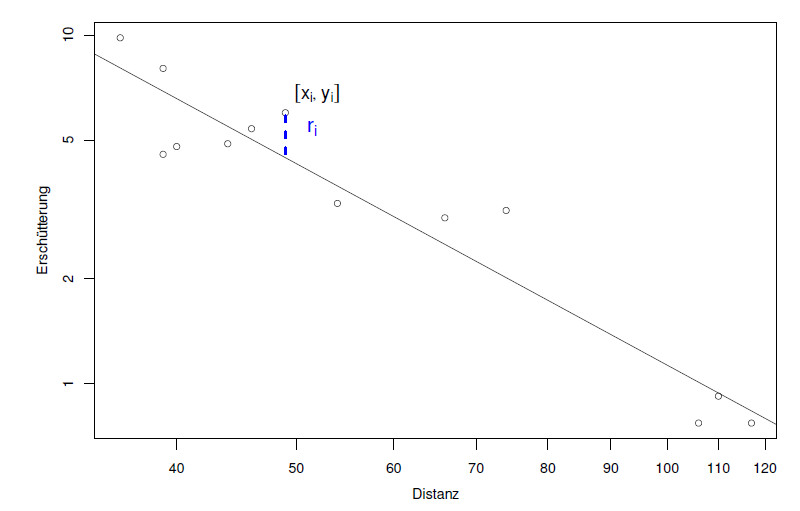
\includegraphics[width=11cm]{pictures/regrFitting.jpg}
}


\frame{\frametitle{Least squares}
For multiple reasons (theoretical aspects and mathematical convenience), the parameters are estimated using the \myalert{least squares} approach. In this, the second type of distances are minimized: \\[6mm]

\colorbox{lightgray}{\begin{minipage}{10cm}
The parameters are estimated such that the sum of \myalert{squared vertical distances}

$$\sum_{i=1}^n r_i^2 \ , \qquad r_i = y_i - (\alpha + \beta x_i) $$

is being minimized.
\end{minipage}}

\vspace{9mm}
Note: The vertical deviations $r_i$ are called the \myalert{residuals}. \\[2mm]


}


\frame{\frametitle{Formulas for regression line parameters}

\colorbox{lightgray}{\begin{minipage}{10cm}
\begin{eqnarray*}
\hat\beta &=& \frac{\sum_{i=1}^n  (y_i - \overline{y}) (x_i - \overline{x})}{ \sum_{i=1}^n (x_i - \overline{x})^2 } = \frac{cov(\bm{x},\bm{y})}{var(\bm{x})} \\[4mm]
\hat\alpha &=& \overline{y} - \hat\beta \overline{x} \\[4mm]
\hat\sigma_E^2 &=& \frac{1}{n-2}\sum_{i=1}^n R_i^2 \quad \text{with residuals  } R_i = y_i - (\hat\alpha - \hat\beta x_i)
\end{eqnarray*}
\end{minipage}}
~\\[6mm]

The hat on the parameters ($\hat\alpha$,$\hat\beta$,$\hat\sigma$) indicates that these are \myalert{estimates}. \\[6mm]

{\small (The derivation of the parameters can be looked up in the Stahel script 2.A b. Idea: Minimization through derivating equations and setting them =0.)}

}



\frame{\frametitle{Do-it-yourself ``by hand''}

Go to the Shiny gallery and try to ``estimate'' the correct parameters.\\[6mm]

You can do this here:\\[2mm]

\url{https://gallery.shinyapps.io/simple_regression/} \\[2mm]


}


\frame[containsverbatim]{\frametitle{Estimation using R}
Let's estimate the regression parameters from the bodyfat example\\[3mm]

%\setkeys{Gin}{width=0.5\textwidth}
\begin{Schunk}
\begin{Sinput}
> r.bodyfat <- lm(bodyfat ~ bmi,d.bodyfat)
> summary(r.bodyfat)
\end{Sinput}
\begin{Soutput}
Call:
lm(formula = bodyfat ~ bmi, data = d.bodyfat)

Residuals:
     Min       1Q   Median       3Q      Max 
-13.5485  -3.5583   0.0785   4.0384  12.7330 

Coefficients:
            Estimate Std. Error t value Pr(>|t|)    
(Intercept) -26.9844     2.7689  -9.746   <2e-16 ***
bmi           1.8188     0.1083  16.788   <2e-16 ***
---
Signif. codes:  0 ‘***’ 0.001 ‘**’ 0.01 ‘*’ 0.05 ‘.’ 0.1 ‘ ’ 1

Residual standard error: 5.573 on 241 degrees of freedom
Multiple R-squared:  0.539,	Adjusted R-squared:  0.5371 
F-statistic: 281.8 on 1 and 241 DF,  p-value: < 2.2e-16
\end{Soutput}
\end{Schunk}

~\\
$\Rightarrow$ $\hat\alpha=-26.98$ ,  $\hat\beta=1.82$, $\hat\sigma_E = 5.57$.\\

Interpretation: for an increase in the bmi by one index point, roughly 1.82\% percentage points more bodyfat are expected.
}


\frame[containsverbatim]{
Plotting the resulting line into the scatterplot is simple:\\[4mm]
\begin{center}
\setkeys{Gin}{width=0.5\textwidth}
\begin{Schunk}
\begin{Sinput}
> plot(bodyfat ~ bmi,d.bodyfat)
> abline(r.bodyfat,lwd=2)
\end{Sinput}
\end{Schunk}
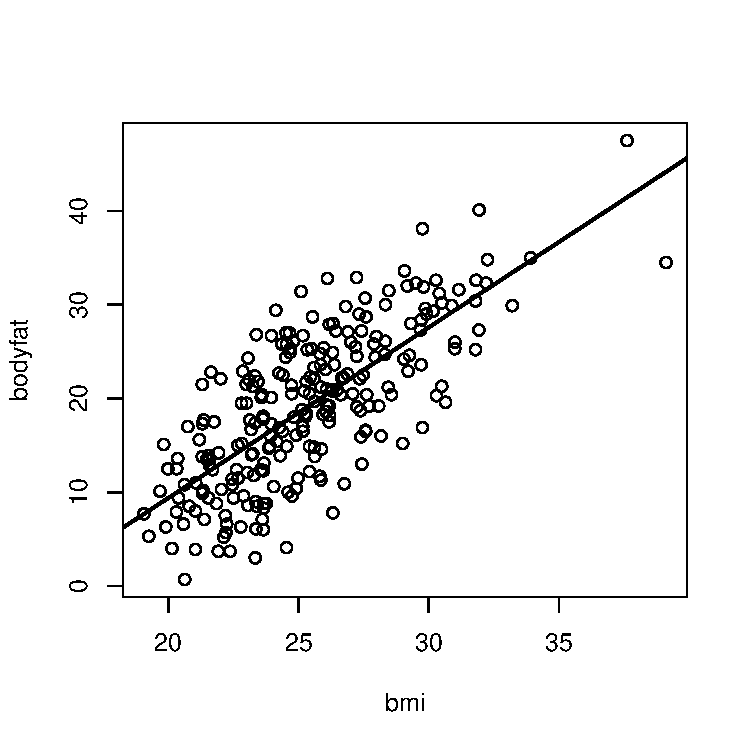
\includegraphics{Bio144_2017_week2-plotbodyfat}
\end{center}

}


\frame[containsverbatim]{\frametitle{Uncertainty in the estimates $\hat\alpha$ and $\hat\beta$}
Let us look again at the regression output, this time only for the coefficients:\\[6mm]

\begin{Schunk}
\begin{Sinput}
> summary(r.bodyfat)$coef
\end{Sinput}
\begin{Soutput}
              Estimate Std. Error   t value     Pr(>|t|)
(Intercept) -26.984368  2.7689004 -9.745518 3.921511e-19
bmi           1.818778  0.1083411 16.787522 2.063854e-42
\end{Soutput}
\end{Schunk}
~\\[6mm]
The second column shows a standard error of the estimate. The estimates thus seem to contain \myalert{uncertainty}!\\[4mm]

The logical next question is: what is the distribution of the estimates?

}



\frame[containsverbatim]{\frametitle{Distribution of $\hat\alpha$ and $\hat\beta$}
\vspace{-6mm}
Again, a simulation can help to get an idea. We generate data points according to the model
%
$$y_i = 4 - 2x_i + E_i \ , \quad E_i\sim \N(0,0.5^2). $$
In each round, we estimate the parameters and store them:\\[3mm]

\begin{Schunk}
\begin{Sinput}
> niter <- 1000
> pars <- matrix(NA,nrow=niter,ncol=2)
> for (ii in 1:niter){
+ x <- rnorm(100)
+ y <- 4 - 2*x + rnorm(100,0,sd=0.5)
+ pars[ii,] <- lm(y~x)$coef
+ }
\end{Sinput}
\end{Schunk}
~\\[2mm]
Doing this \numprint{1000} times, we obtain the following distributions for $\hat\alpha$ and $\hat\beta$.
}

\frame[containsverbatim]{\label{sl:dists}
\setkeys{Gin}{width=0.85\textwidth}
\begin{Schunk}
\begin{Sinput}
> par(mfrow=c(1,2))
> hist(pars[,1],xlab =expression(alpha),main="",freq=F,nclass=20)
> hist(pars[,2],xlab=expression(beta),main="",freq=F,nclass=20)
\end{Sinput}
\end{Schunk}
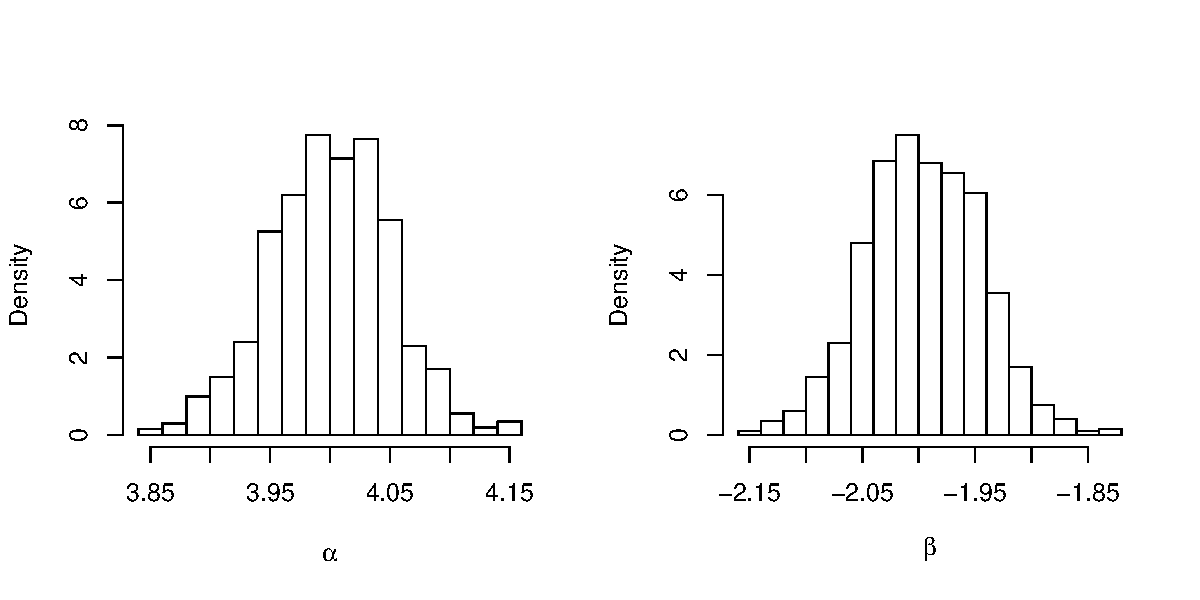
\includegraphics{Bio144_2017_week2-010}

This looks suspiciously normal... \\[2mm]
In fact, from theory:
\begin{eqnarray*}
\hat\beta \sim \N(\beta,{\sigma^{(\beta)2}}) & \quad \text{and} \quad & \hat\alpha \sim \N(\alpha,{\sigma^{(\alpha)2}})
\end{eqnarray*}
}

\frame{
The standard deviations ${\sigma^{(\beta)2}}$ and ${\sigma^{(\alpha)2}}$ are defined as

$$\sigma^{(\beta)2} = \sigma_E^2 / \text{SSQ}^{(X)} \qquad \sigma^{(\alpha)2} = \sigma_E^2 \left(\frac{1}{n} + \overline{x}^2/\text{SSQ}^{(X)}\right)$$

with the sum-of-squares for $X$ given as
$$\text{SSQ}^{(X)} = \sum_{i=1}^n (x_i-\overline{x})^2 \ .$$

{\small(See also Stahel 2.2.h)}\\[2mm]

Don't worry, you do not need to know these formulas by heart! \\[3mm]

\colorbox{lightgray}{\begin{minipage}{10cm}
{\bf You should know that}
\begin{itemize}
\item the parameters estimates $\hat\alpha$ and $\hat\beta$ are \myalert{normally distributed.}
\item the formulas to calculate the variances depend on the residual variance $\sigma_E^2$, the sample size $n$ and SSQ$^{(X)}$.
\end{itemize}
\end{minipage}}
}



\frame[containsverbatim]{\frametitle{How good is the regression model?}
This is, per se, a difficult question.... \\[2mm]

One often considered index is the {\bf coefficient of determination (Bestimmtheitsmass)} $R^2$.
Let us again look at the regression output form the bodyfat example:\\[4mm]

\begin{Schunk}
\begin{Sinput}
> summary(r.bodyfat)$r.squared
\end{Sinput}
\begin{Soutput}
[1] 0.5390391
\end{Soutput}
\end{Schunk}

~\\[0mm]
This is the $R^2$ from the regression of bodyfat against bmi. \\
Compare this to the correlation between the two variables:\\[2mm]

\begin{Schunk}
\begin{Sinput}
> cor(d.bodyfat$bodyfat,d.bodyfat$bmi)
\end{Sinput}
\begin{Soutput}
[1] 0.7341928
\end{Soutput}
\end{Schunk}
~\\
... and square it:\\[2mm]
\begin{Schunk}
\begin{Sinput}
> cor(d.bodyfat$bodyfat,d.bodyfat$bmi)^2
\end{Sinput}
\begin{Soutput}
[1] 0.5390391
\end{Soutput}
\end{Schunk}
}

\frame{

We conclude:\\[2mm]

\colorbox{lightgray}{\begin{minipage}{10cm}
In simple linear regression, $R^2$ is the squared correlation between the independent and the dependent variable.
\end{minipage}}\\[6mm]


Generally, $R^2$ indicates the proportion of variability of the response variable $\bm{y}$ that is explained by the ensemble of all covariates. {\bf The larger $R^2$, the more variability of $\bm{y}$ is captured by the covariates, thus the ``better'' is the model.} (However, we will qualify this statement later in the course...)\\[6mm]

$R^2$ becomes more interesting in \emph{multiple} linear regression.\\

}

\frame{\frametitle{Testing and Confidence Intervals}\label{sl:testsCI}
After the regression parameters and their uncertainties have been estimated, there are typically two fundamental questions to be answered:\\[4mm]

\begin{enumerate}
\item {\bf ''Are the parameters compatible with some specific value?''} \\
Typically, the question is whether the slope $\beta$ might be 0 or not, that is: ``Is there an effect of the covariate $\bm{x}$ or not?''\\
$\Rightarrow$ This leads to a {\bf statistical test}.\\[4mm]

\item {\bf ``Which values of the parameters are compatible with the data?''}\\
$\Rightarrow$ This leads us to determine {\bf confidence intervals}.\\[4mm]
\end{enumerate}
}

\frame[containsverbatim]{
Let's first go back to the output from the bodyfat example:\\[5mm]
\begin{Schunk}
\begin{Sinput}
> summary(r.bodyfat)$coef
\end{Sinput}
\begin{Soutput}
              Estimate Std. Error   t value     Pr(>|t|)
(Intercept) -26.984368  2.7689004 -9.745518 3.921511e-19
bmi           1.818778  0.1083411 16.787522 2.063854e-42
\end{Soutput}
\end{Schunk}
~\\[4mm]
Besides the estimate and the standard error (which we discussed before), there is a t value and a probability Pr(>|t|) that we need to understand. \\[2mm]

How do these things help us to answer the two questions above?
}


\frame{\frametitle{Testing the effect of a covariate}
Remember: in a statistical test you first need to specify the \emph{null hypothesis}. Here, typically, the null hypothesis is
$$H_0: \quad \beta = \beta_0 =  0  \ .$$
Included in $H_0$ is the assumption that the data follow the simple linear regression model. \\
{\small (However, you might want to test against another null hypothesis, see Stahel 2.3 a,b).}\\[2mm]

Here, the \emph{alternative hypothesis} is given by
$$H_A: \quad \beta \neq  0  \ ,$$

 }
 
\frame{
Remember: to carry out a statistical test, we need a \emph{test statistic}.\\[4mm]

What is a test statistic?? (Clicker exercise here?)\\[6mm]

\pause

It is some type of summary statistic that follows a known distribution under $H_0$. For our purpose, we use the so-called $T$-statistic\\[4mm]

\colorbox{lightgray}{\begin{minipage}{10cm}
\begin{equation}\label{eq:beta}
T=\frac{\hat\beta - \beta_0}{se^{(\beta)}} \quad \text{with} \quad se^{(\beta)}=\sqrt{\hat\sigma_E^2/SSQ^{(X)}}  \ .
\end{equation}
\end{minipage}}

~\\[2mm]
Again: typically, $\beta_0=0$, so the formula simplifies to.... (please think:-))\\[2mm]

Under $H_0$, $T$ has a $t$-distribution with $n-2$ degrees of freedom ($n=$ number of data points).\\
(Question: do you remember why this is a t-distribution? Check Mat183, keyword: t-test.)

}


\frame[containsverbatim]{
So let's again go back to the bodyfat regression output:\\[4mm]

\begin{Schunk}
\begin{Sinput}
> summary(r.bodyfat)$coef
\end{Sinput}
\begin{Soutput}
              Estimate Std. Error   t value     Pr(>|t|)
(Intercept) -26.984368  2.7689004 -9.745518 3.921511e-19
bmi           1.818778  0.1083411 16.787522 2.063854e-42
\end{Soutput}
\end{Schunk}
~\\[6mm]

2 tasks:
\begin{enumerate}
\item Please use equation \eqref{eq:beta} to find out how the first three columns (Estimate, Std. Error and t value) are related! Check your ideas by doing some calculations...\\[7mm]
\item Then think how we get the fourth column from the third. \\
Hint: last column contains the {\bf $p$-value} of the test $\beta=0$.\\[2mm]
\end{enumerate}
}

\frame[containsverbatim]{
For task 2 above we can use the built-in ``distribution table'' of the t-distribution in R:\\[2mm]

\begin{Schunk}
\begin{Sinput}
> 2*pt(16.787522,241,lower.tail=F)
\end{Sinput}
\begin{Soutput}
[1] 2.063861e-42
\end{Soutput}
\end{Schunk}
~\\[6mm]
Conclusion: there is very strong evidence that the BMI is associated with bodyfat, because $p$ is extremely small.\\[4mm]

This basically answers question 1 from slide \ref{sl:testsCI}.\\[6mm]

\textcolor{gray}{\small (Remark: if you forgot the details of the $p$-value, I have a special task for you: go back to the book ``Statistische Datenanalyse'' from W. Stahel and read chapter 8.7.)}
}


\frame[containsverbatim]{\frametitle{A cautionary note on the use of $p$-values}
Maybe you have seen that in statistical testing, often the criterion $p\leq 0.05$ is used to test whether $H_0$ should be rejected. This is often done in a black-or-white manner.\\[4mm]

\colorbox{lightgray}{\begin{minipage}{10cm}
However, we will put a lot of attention to a more reasonable and cautionary interpretation of $p$-values in this course! 
\end{minipage}}
}

% \frame{
% Question: On slide \ref{sl:dists} we have seen that $\hat\beta \sim \N(\beta,{\sigma^{(\beta)2}})$. So why does $T$ in equation \eqref{eq:beta} follow a $t$-distribution, and not a normal distribution? \\[4mm]
% 
% Remember: In Mat183 you have learned that when the variance $\sigma^2_E$ in the formula is replaced by its estimate $\hat\sigma^2_E$, then the normal distribution must be replaced by the $t$-distribution (Keyword: t-test).
% 
% }


\frame{\frametitle{Confidence intervals of regression parameters}
Question 2 from slide \ref{sl:testsCI}: ``Which values of the parameters are compatible with the data?''\\[4mm]

To answer this question, we can determine the confidence intervals of the regression parameters.\\[4mm]

Let us collect the facts we know about $\hat\beta$:
\begin{itemize}
\item $\hat\beta$ is estimated with a standard error of $\sigma^{(\beta)}$.
\item The distribution of $\hat\beta$ is normal, namely $\hat\beta\sim\N(\beta,\sigma^{(\beta)2})$.
\item However, since we need to estimate $\sigma_E^2$ from the data, we have a $t$-distribution.
\end{itemize}
}

\frame[containsverbatim]{
Doing some calculations (blackboard) leads us to the 95\% confidence interval\\[2mm]

\begin{center}
\colorbox{lightgray}{\begin{minipage}{6cm}
$$[\hat\beta - c \cdot \sigma^{(\beta)} ; \hat\beta + c \cdot \sigma^{(\beta)}] \ ,$$
\end{minipage}}
\end{center}
~\\[1mm]

where $c$ is the 97.5\% quantile of the $t$-distribution with $n-2$ degrees of freedom. \\[2mm]

Doing this for the bodfat example ``by hand'' is not hard. We have 241 degrees of freedom:\\[4mm]
\begin{Schunk}
\begin{Sinput}
> coefs <- summary(r.bodyfat)$coef
> beta <- coefs[2,1]
> sdbeta <- coefs[2,2] 
> beta + c(-1,1) * qt(0.975,241) * sdbeta 
\end{Sinput}
\begin{Soutput}
[1] 1.605362 2.032195
\end{Soutput}
\end{Schunk}
~\\[2mm]

}

\frame[containsverbatim]{
Even easier: directly ask R to give you the CIs.\\[2mm]

\begin{Schunk}
\begin{Sinput}
> confint(r.bodyfat,level=c(0.95))
\end{Sinput}
\begin{Soutput}
                 2.5 %     97.5 %
(Intercept) -32.438703 -21.530032
bmi           1.605362   2.032195
\end{Soutput}
\end{Schunk}
~\\[8mm]
\underline{Interpretation:} all true values for $\beta$ between 1.61 and 2.03 are compatible with the observed data.


%' ~\\[5mm]
%' Note that you can also choose another level than 95\%, for instance 90\%:\\[2mm]
%' 
%' <<echo=T,eval=T>>=
%' confint(r.bodyfat,level=c(0.90))
%' @
}



\frame{\frametitle{Confidence and Prediction Ranges}
\begin{itemize}
\item Remember: When another sample from the same population was taken, the regression line would look slightly different.\\[4mm]
\item There are two questions to be asked:\\[6mm]
\end{itemize}

\begin{enumerate}
\item Which other regression lines are compatible with the observed data?\\[2mm]
$\Rightarrow$ This leads to the {\bf confidence range}. \\[4mm]
\item Where do future observations with a given $x$ coordinate lie? \\[2mm]
$\Rightarrow$ This leads to the {\bf prediction range}.
\end{enumerate}
}


\frame{\frametitle{Bodyfat example}
\vspace{-5mm}
\begin{center}
\setkeys{Gin}{width=0.65\textwidth}
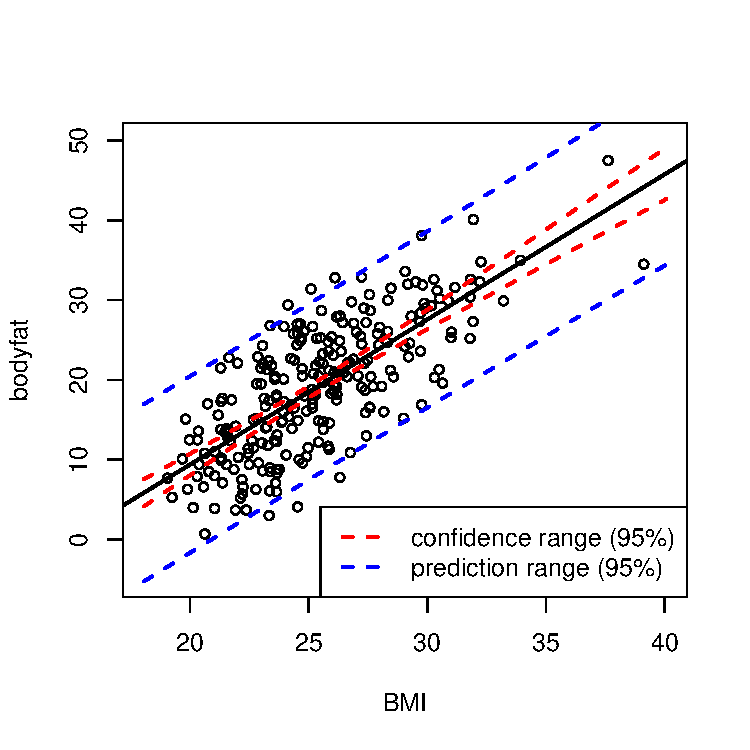
\includegraphics{Bio144_2017_week2-confpred}
\end{center}

Note: The prediction range is much broader than the confidence range.
}


\frame{\frametitle{Calculation of the confidence range}
Given a fixed value of $x$, say $x_0$. The question is: \\[2mm]

\colorbox{lightgray}{\begin{minipage}{10cm}
Where does $\hat y_0 = \hat\alpha + \hat\beta x_0$ lie with a certain confidence (i.e., 95\%)? 
\end{minipage}}\\[2mm]

This question is not trivial, because both $\hat\alpha$ and $\hat\beta$ are estimates from the data and contain uncertainty. \\[2mm]

The details of the calculation are given in Stahel 2.4b. (Idea: $\hat y_0 \pm q\cdot se^{(y_0)}$.) \\[6mm]

\colorbox{lightgray}{\begin{minipage}{10cm}
For \emph{each} $x_0$ one obtains a confidence interval for the expected value $\hat y_0 = \hat\alpha + \hat\beta x_0$. Plotting this interval for all values of $x_0$ one obtains the {\bf confidence range} or {\bf confidence band for the expected values} of $y$.
\end{minipage}}\\[2mm]


Note: For the confidence range, only the uncertainty in the estimates $\hat\alpha$ and $\hat\beta$ are decisive.
}


\frame{
\vspace{-5mm}
\begin{center}
\setkeys{Gin}{width=0.65\textwidth}
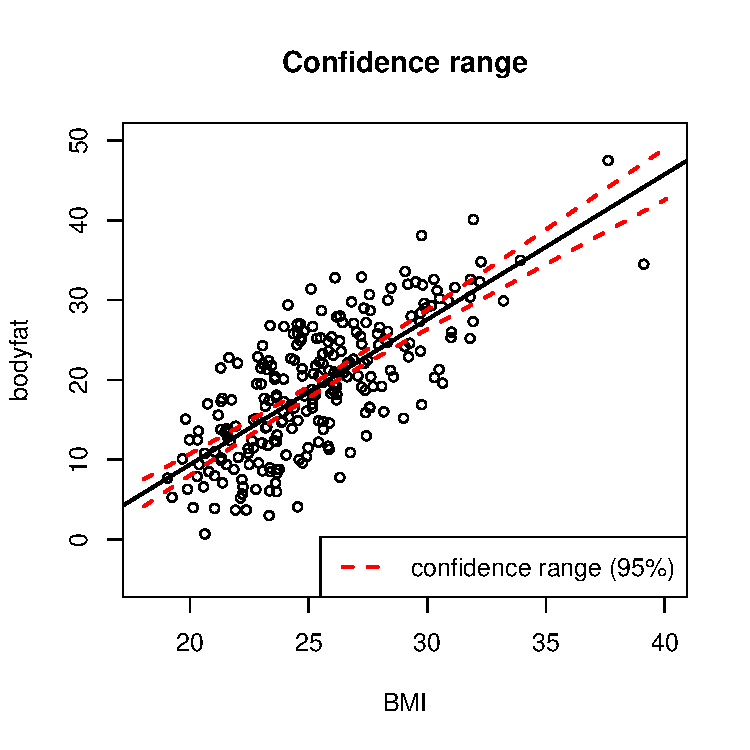
\includegraphics{Bio144_2017_week2-conf}
\end{center}

}



\frame{\frametitle{Calculation of the prediction range}
Given a fixed value of $x$, say $x_0$. The question is: \\[6mm]

\colorbox{lightgray}{\begin{minipage}{10cm}
Where does a {\bf future observation} lie with a certain confidence (i.e., 95\%)? 
\end{minipage}}\\[6mm]

To answer this question, we have to consider not only the uncertainty in the predicted value $\hat y_0 =  \hat\alpha + \hat\beta x_0$, but also the error in the equation $E_i \sim \N(0,\sigma_E^2)$. \\[6mm]


This is the reason why the prediction range is always wider than the confidence range.

}


\frame{
\vspace{-5mm}
\begin{center}
\setkeys{Gin}{width=0.65\textwidth}
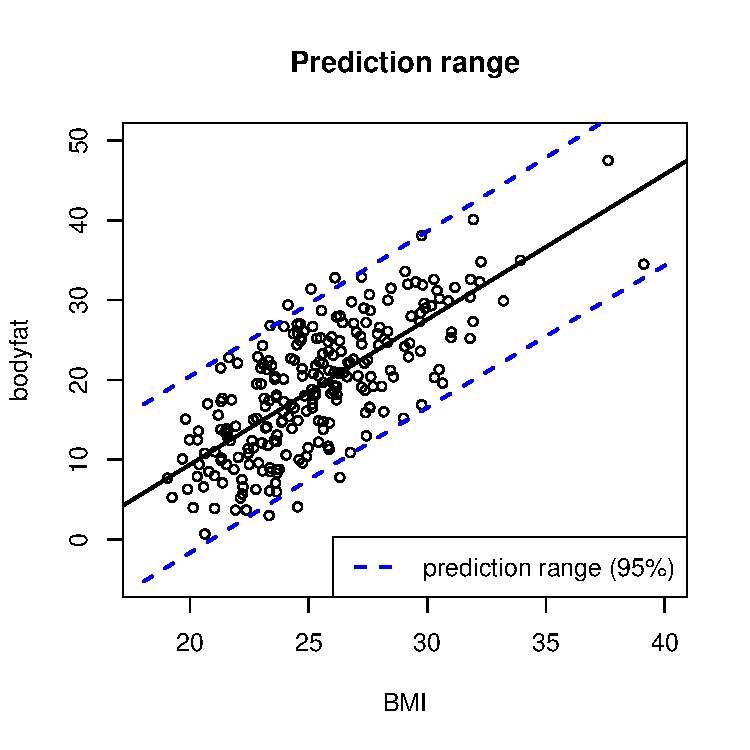
\includegraphics{Bio144_2017_week2-pred}
\end{center}

}



\frame{\frametitle{Further reading}

``Points of significance: Simple linear regression'' is a nice, 2-page overview of simple linear regression, summarized in Nature Methods in 2015:\\[4mm]



\url{http://www.nature.com/nmeth/journal/v12/n11/full/nmeth.3627.html}
}

\frame{\frametitle{Summary}

}

%\frame{References:
%\bibliographystyle{Chicago}
%\bibliography{refs}
%}

\end{document}
